\section{Results}

This section reports the \gls{NSLKDD} multiplicity run described in Section~III. The experiment trained 15 neural classifiers from five random seeds and three stratified training-subset fractions. Accuracy ranges from 0.769 to 0.799, while macro-\gls{F1} ranges from 0.769 to 0.799. The best model is \texttt{seed5\_frac0p75} with an accuracy of 0.799 and a macro-\gls{F1} score of 0.799. Models trained on 75\% of the training data perform best on average, with a mean accuracy of 0.793, compared with 0.785 for the full-data models and 0.780 for the 50\% subset models.

\begin{figure}[t]
    \centering
    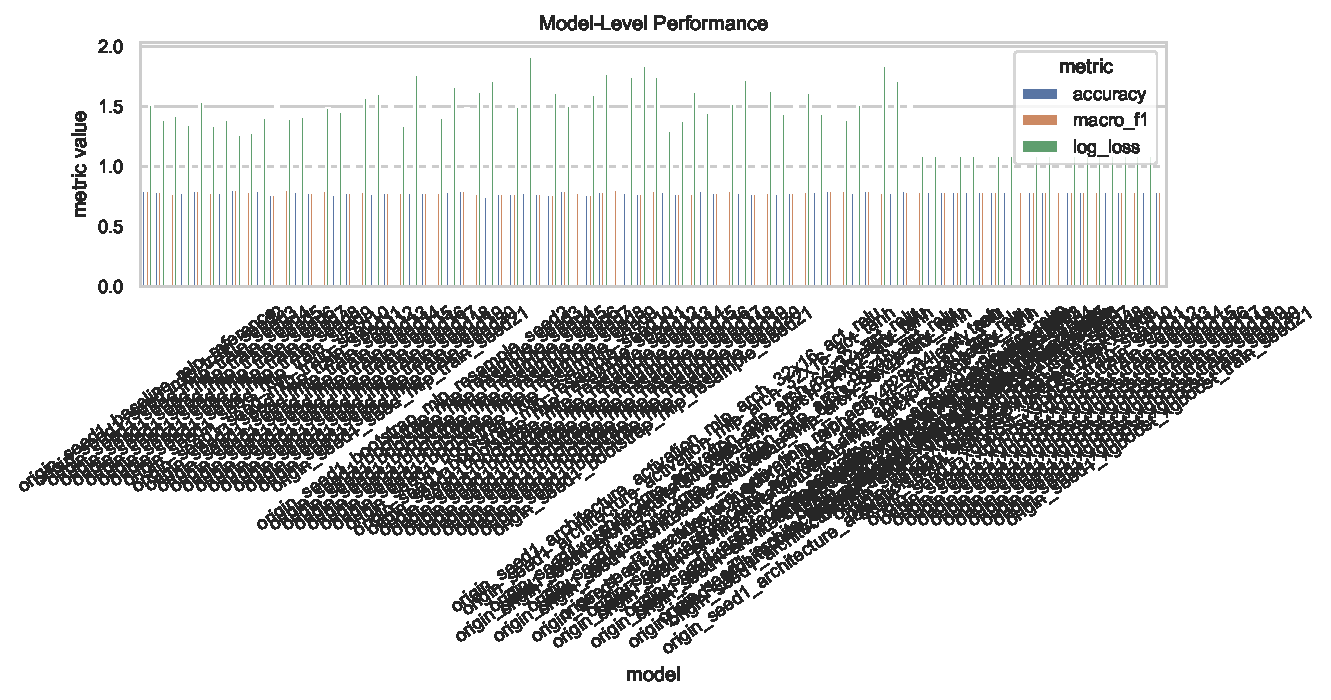
\includegraphics[width=\columnwidth]{figures/results_metrics_by_model.pdf}
    \caption{Predictive performance of all 15 candidate models. The models are close in aggregate metrics, with the best accuracy observed for \texttt{seed5\_frac0p75}.}
    \label{fig:results_metrics_by_model}
\end{figure}

\begin{figure}[t]
    \centering
    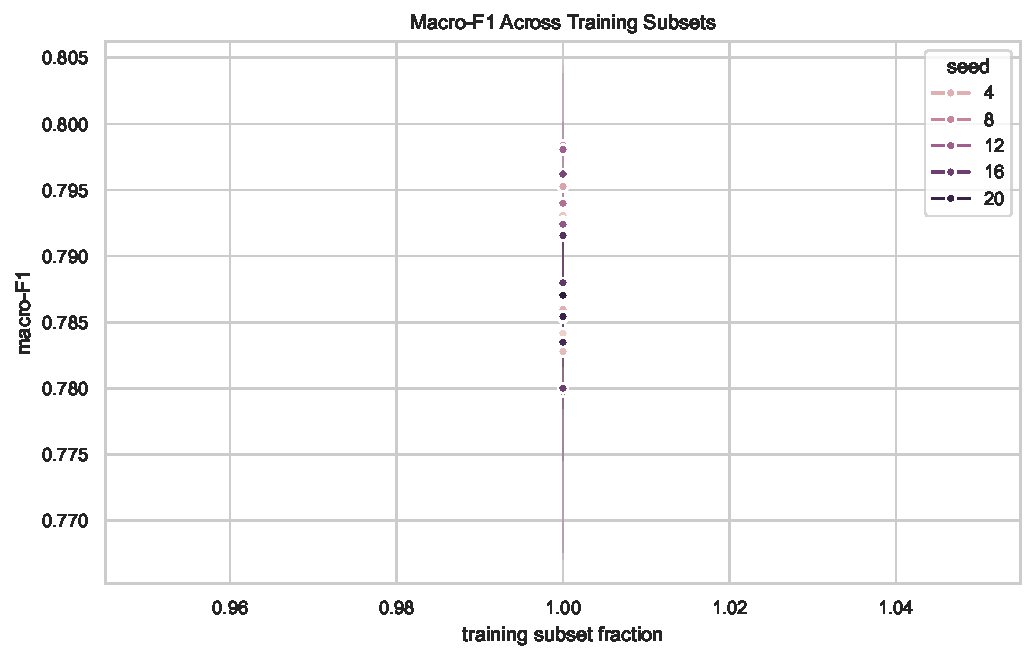
\includegraphics[width=\columnwidth]{figures/results_macro_f1_by_subset.pdf}
    \caption{Macro-\gls{F1} by training-subset fraction. The 75\% subset models have the strongest average performance in the current run.}
    \label{fig:results_macro_f1_by_subset}
\end{figure}

\subsection{Rashomon Set and Predictive Multiplicity}

Using accuracy as the Rashomon metric with tolerance $\epsilon=0.015$, 10 of the 15 candidate models are retained in the Rashomon set. This shows that the training procedure produces several models with nearly indistinguishable aggregate performance. The predictive metrics alone therefore do not identify a unique best model.

The Rashomon-set models nevertheless differ on individual test samples. Across all model pairs in the Rashomon set, the mean pairwise disagreement rate is 0.035, with a maximum pairwise disagreement of 0.060. The sample-level ambiguity is 0.100, meaning that about 10\% of test samples receive more than one predicted label across the retained models. The mean conflict ratio is 0.022 and the maximum conflict ratio is 0.5. Thus, although most samples are classified consistently, a non-negligible subset remains locally underdetermined by model selection.

\begin{figure}[t]
    \centering
    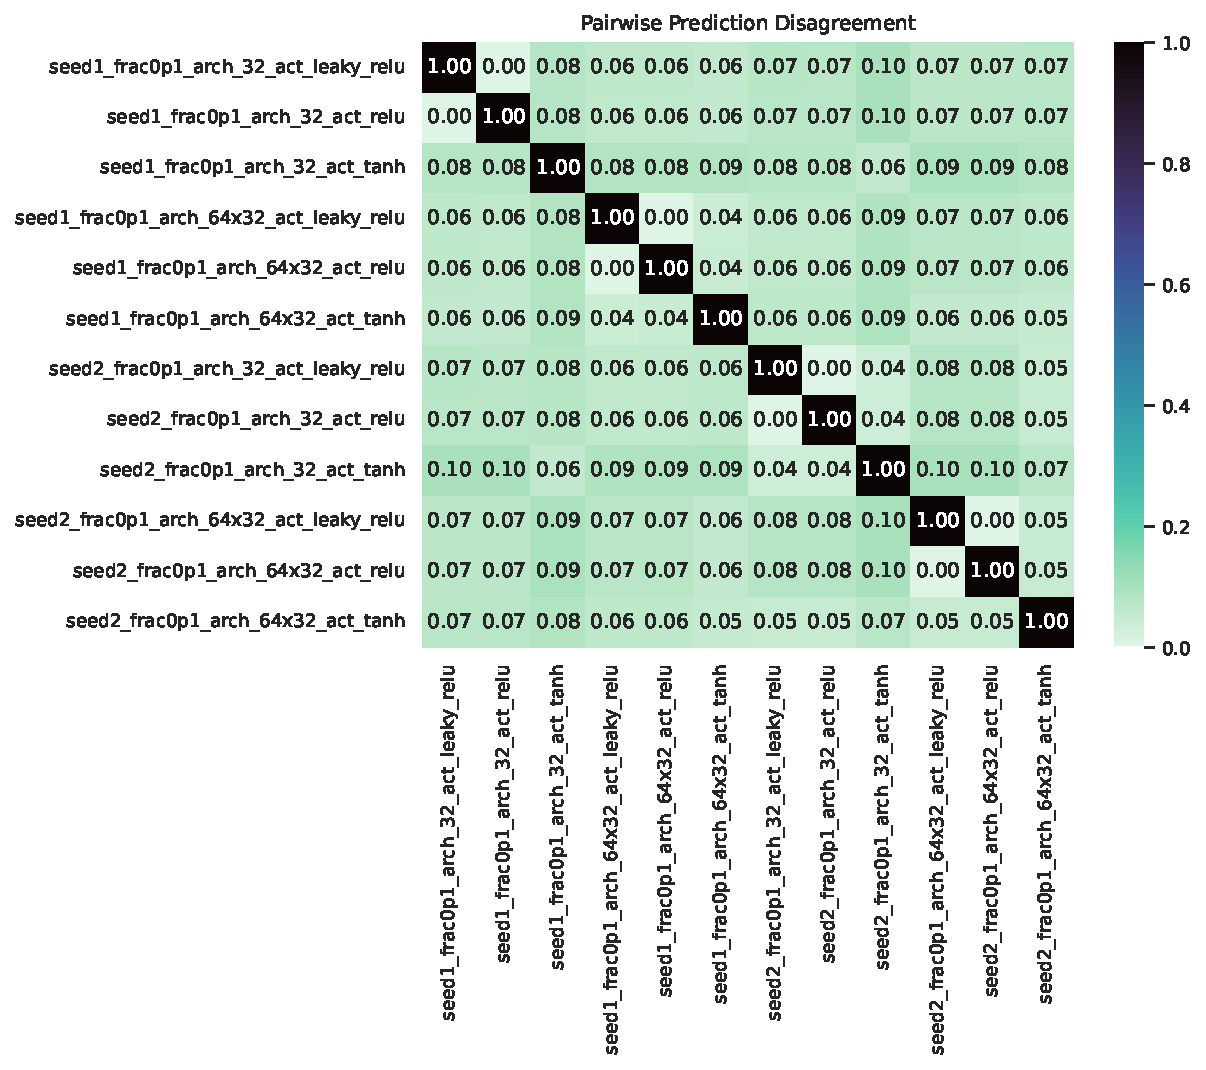
\includegraphics[width=\columnwidth]{figures/results_decision_disagreement_heatmap.pdf}
    \caption{Pairwise predictive disagreement between Rashomon-set models. The strongest disagreement occurs between models that still satisfy the same performance tolerance.}
    \label{fig:results_decision_disagreement}
\end{figure}

\begin{figure}[t]
    \centering
    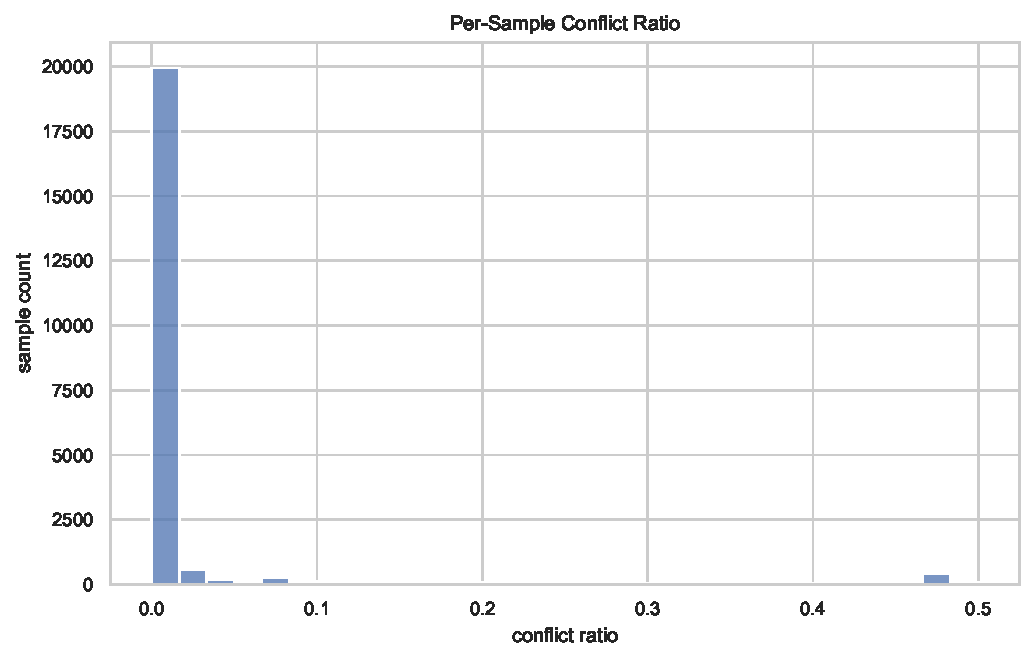
\includegraphics[width=\columnwidth]{figures/results_conflict_ratio.pdf}
    \caption{Distribution of pointwise conflict ratios across the test set. Most samples are stable, but a subset receives conflicting predictions across similarly accurate models.}
    \label{fig:results_conflict_ratio}
\end{figure}

The largest disagreement occurs between \texttt{seed1\_frac1p0} and \texttt{seed3\_frac0p75}, which disagree on 6.0\% of the 22,544 test samples. Several of the largest disagreements involve \texttt{seed3\_frac0p75}, suggesting that even models inside the same Rashomon set can occupy different regions of the solution space.

\subsection{Feature Importance and Explanation Disagreement}

The \gls{SHAP} summaries show that both classes are dominated by host-level traffic statistics. Averaged across Rashomon-set models, the most important attack-class features are \texttt{num\_\_dst\_host\_same\_src\_port\_rate}, \texttt{num\_\_dst\_host\_same\_srv\_rate}, \texttt{num\_\_dst\_host\_srv\_count}, \texttt{num\_\_dst\_host\_diff\_srv\_rate}, and \texttt{num\_\_dst\_host\_rerror\_rate}. The normal class has a similar leading feature set, headed by \texttt{num\_\_dst\_host\_same\_src\_port\_rate}, \texttt{num\_\_dst\_host\_same\_srv\_rate}, and \texttt{num\_\_dst\_host\_srv\_count}. This indicates that the models rely heavily on aggregate destination-host behavior rather than only on per-connection attributes.

\begin{figure*}[t]
    \centering
    \begin{subfigure}[t]{0.48\textwidth}
        \centering
        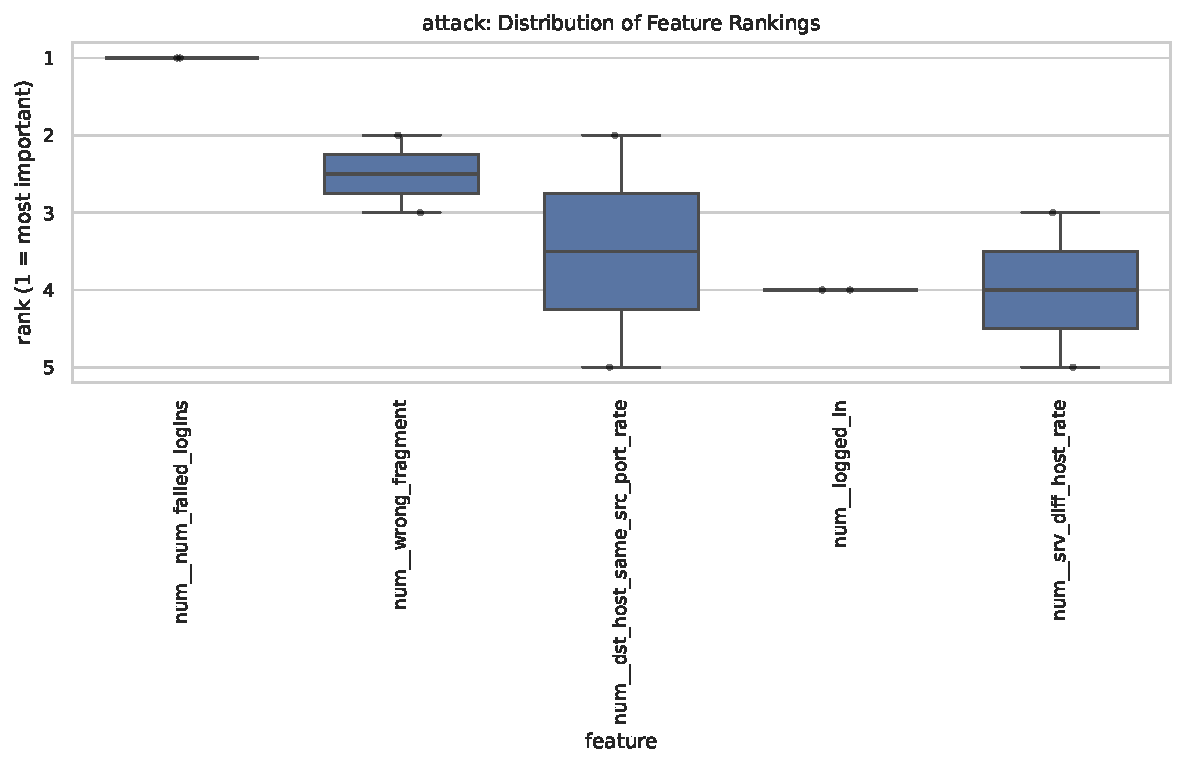
\includegraphics[width=\linewidth]{figures/results_feature_ranking_attack.pdf}
        \caption{Attack class}
        \label{fig:results_feature_ranking_attack}
    \end{subfigure}
    \hfill
    \begin{subfigure}[t]{0.48\textwidth}
        \centering
        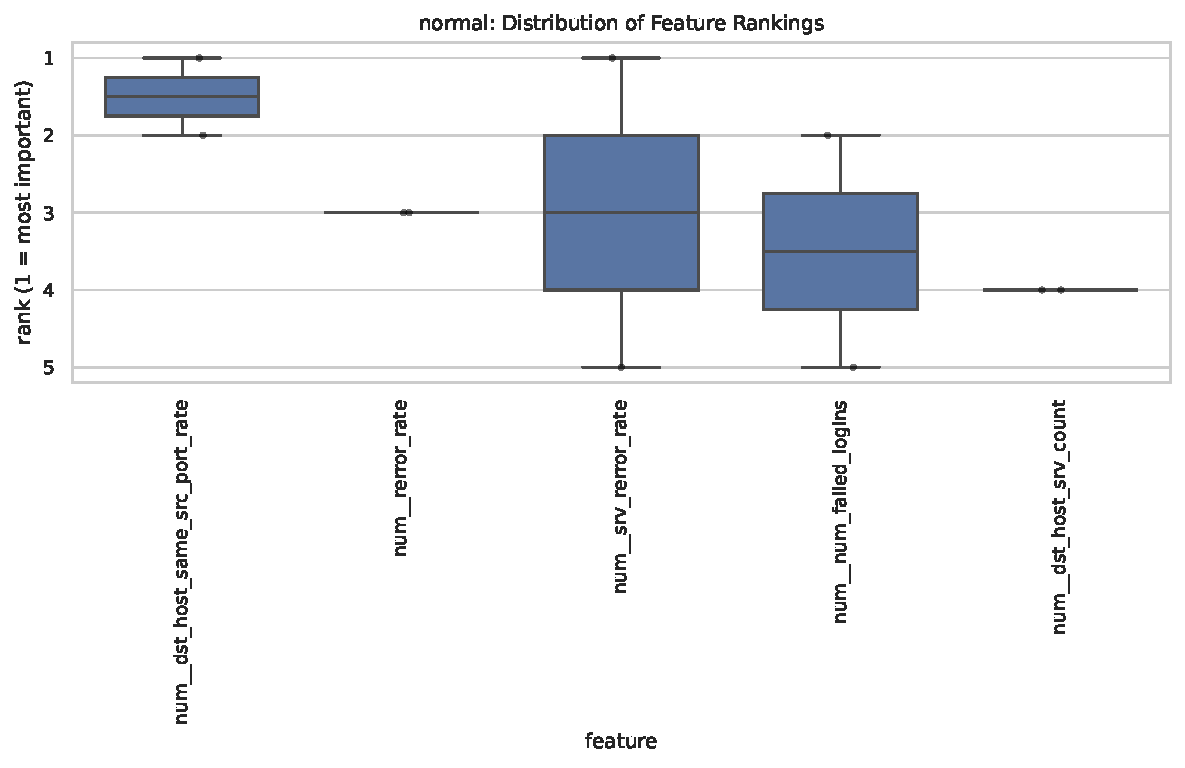
\includegraphics[width=\linewidth]{figures/results_feature_ranking_normal.pdf}
        \caption{Normal class}
        \label{fig:results_feature_ranking_normal}
    \end{subfigure}
    \caption{Aggregated \gls{SHAP} feature rankings across Rashomon-set models. Both classes are dominated by destination-host traffic statistics.}
    \label{fig:results_feature_rankings}
\end{figure*}

Although the same broad feature families appear across models, the explanation comparison reveals measurable attribution variability. The mean cosine distance between mean absolute \gls{SHAP} vectors is 0.066 for the attack class and 0.069 for the normal class. The maximum observed cosine distance is 0.139 for attack and 0.136 for normal. Top-\(20\) feature-set overlap is moderate to high, with mean Jaccard overlaps of 0.710 for attack and 0.716 for normal. In other words, models tend to agree on many important features, but their attribution magnitudes and rankings are not identical.

\begin{figure*}[t]
    \centering
    \begin{subfigure}[t]{0.48\textwidth}
        \centering
        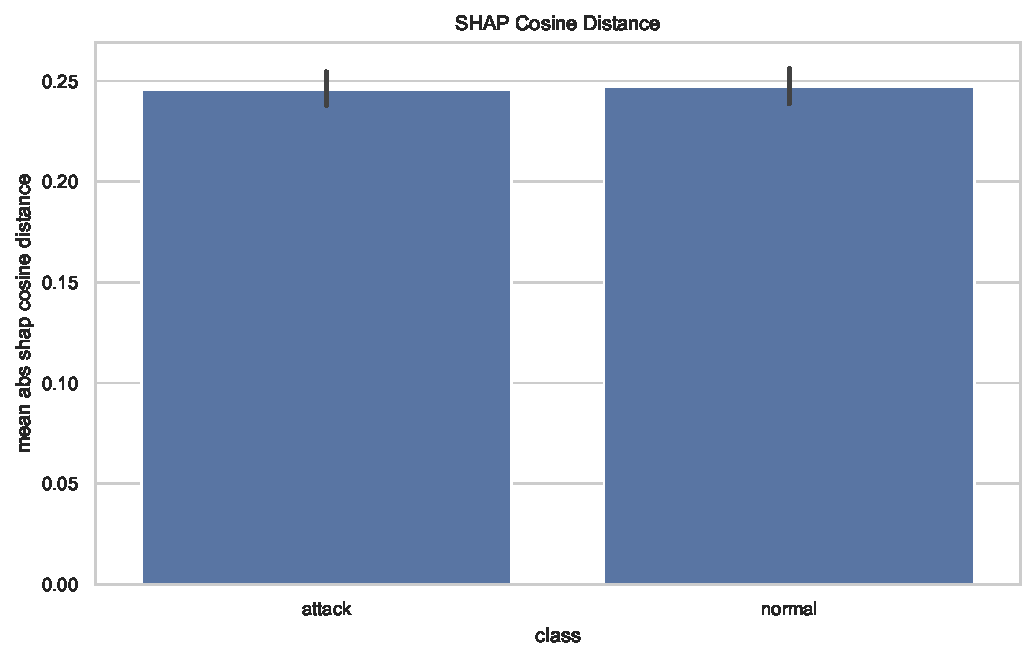
\includegraphics[width=\linewidth]{figures/results_explanation_cosine_distance.pdf}
        \caption{Cosine distance}
        \label{fig:results_explanation_cosine}
    \end{subfigure}
    \hfill
    \begin{subfigure}[t]{0.48\textwidth}
        \centering
        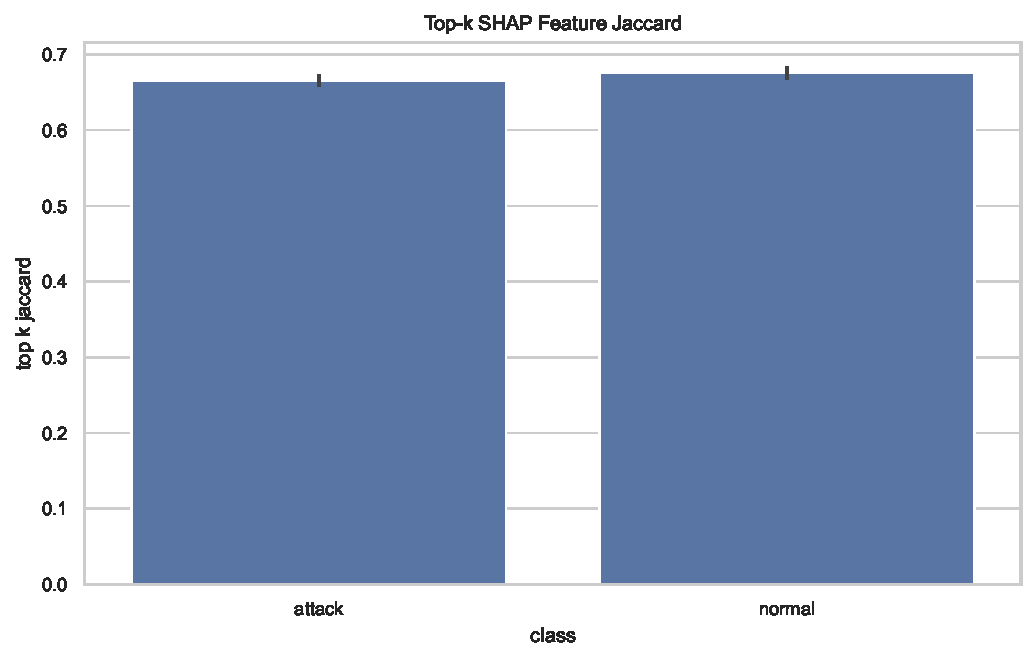
\includegraphics[width=\linewidth]{figures/results_explanation_topk_jaccard.pdf}
        \caption{Top-\(k\) Jaccard overlap}
        \label{fig:results_explanation_jaccard}
    \end{subfigure}
    \caption{Pairwise explanation disagreement between Rashomon-set models. The retained models share many important features, but attribution vectors and rankings still vary.}
    \label{fig:results_explanation_disagreement}
\end{figure*}

\subsection{Explanation Variability on Conflicted Samples}

The conflict-focused explanation analysis covers 256 samples and compares \gls{SHAP} values across Rashomon-set models. The largest mean \gls{SHAP} ranges occur for \texttt{num\_\_srv\_count}, \texttt{num\_\_count}, \texttt{num\_\_dst\_host\_diff\_srv\_rate}, \texttt{num\_\_dst\_host\_serror\_rate}, \texttt{num\_\_dst\_host\_count}, and \texttt{num\_\_dst\_host\_same\_srv\_rate}. Several of these features are also among the globally important \gls{SHAP} features, which means that explanation instability affects features that would plausibly be inspected by an analyst.

\begin{figure*}[t]
    \centering
    \begin{subfigure}[t]{0.48\textwidth}
        \centering
        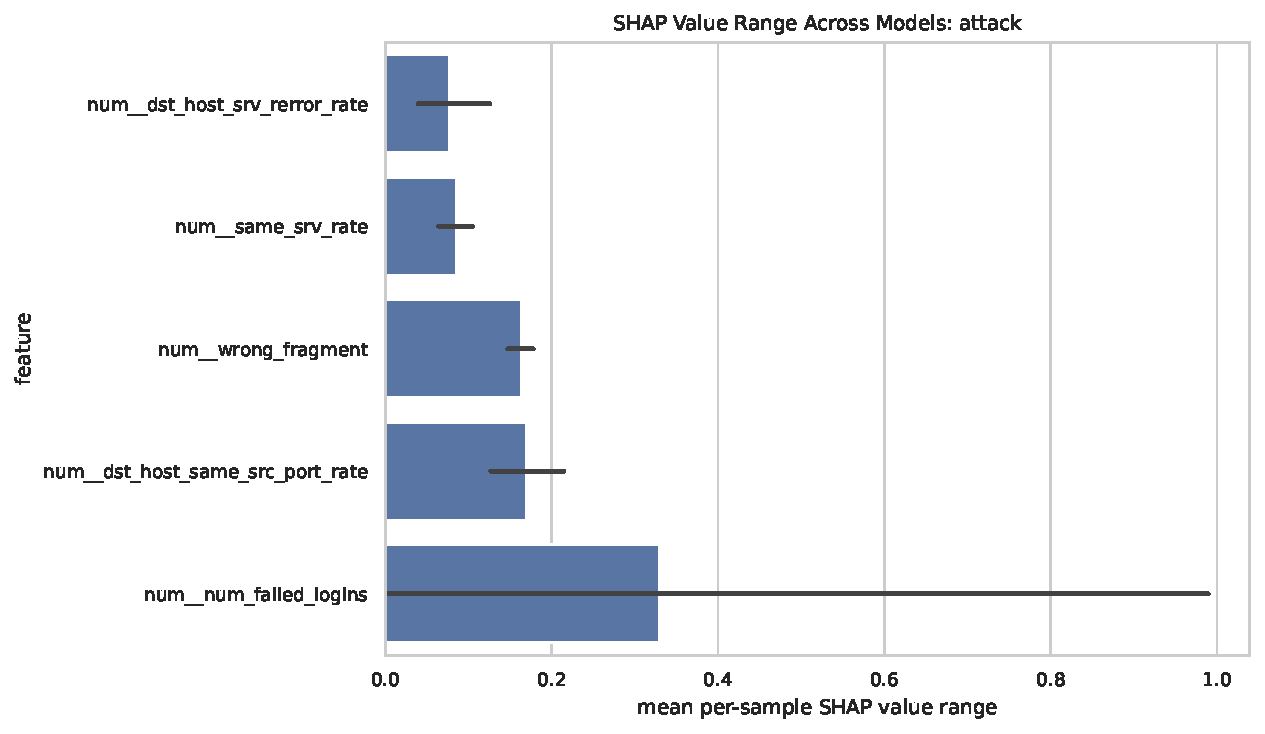
\includegraphics[width=\linewidth]{figures/results_shap_value_range_attack.pdf}
        \caption{\gls{SHAP} range, attack class}
        \label{fig:results_shap_range_attack}
    \end{subfigure}
    \hfill
    \begin{subfigure}[t]{0.48\textwidth}
        \centering
        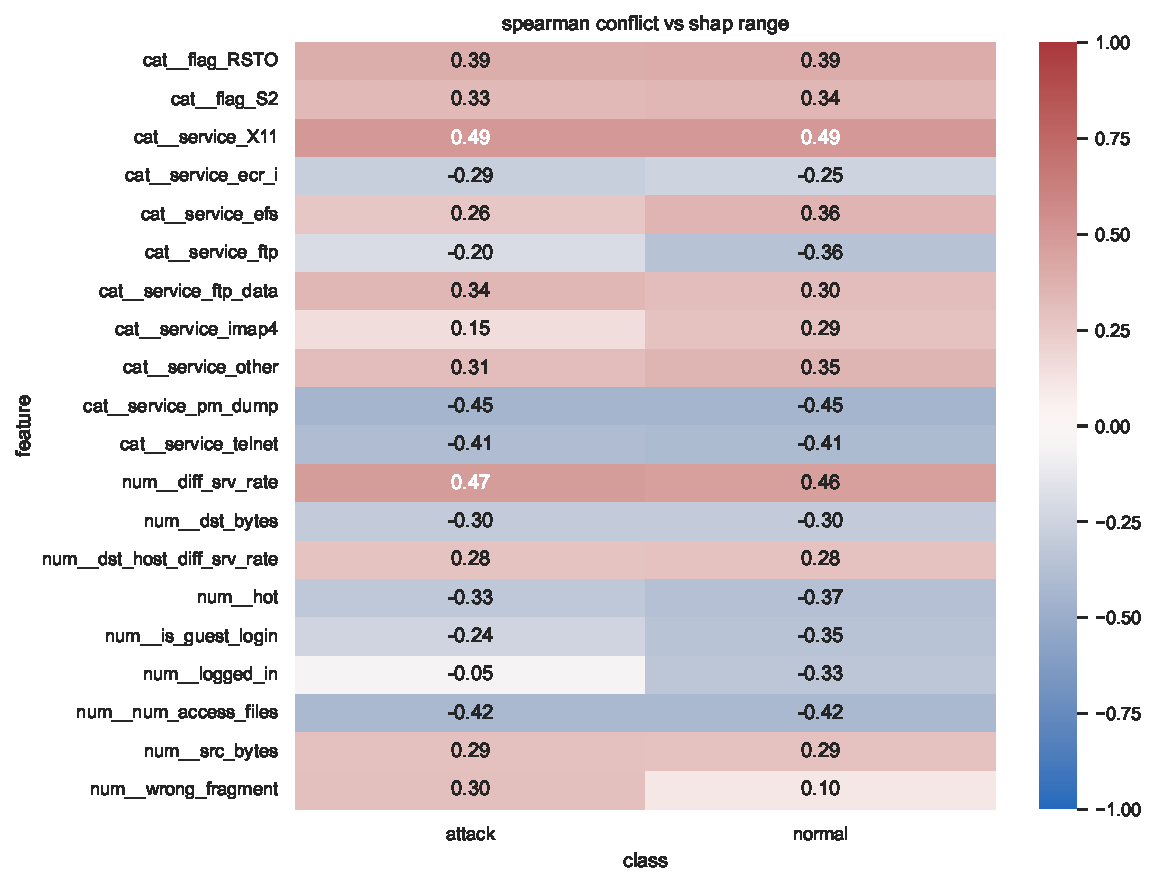
\includegraphics[width=\linewidth]{figures/results_spearman_conflict_shap_range.pdf}
        \caption{Conflict-range correlation}
        \label{fig:results_spearman_conflict_range}
    \end{subfigure}
    \caption{Explanation variability on conflict-focused samples. Important features can exhibit substantial attribution ranges, while correlations between predictive conflict and \gls{SHAP} range remain moderate.}
    \label{fig:results_explanation_variability}
\end{figure*}

The correlations between predictive conflict and \gls{SHAP} variability are present but not dominant. The strongest absolute Spearman correlations between conflict ratio and \gls{SHAP} range are around 0.33. This suggests that predictive disagreement and explanation variability are related, but not interchangeable: some features can show unstable attributions even when the conflict signal is modest, and conflict can arise without a uniformly large change in every feature attribution.

\subsection{Summary}

Overall, the results support the central claim that aggregate performance is insufficient for assessing model stability in intrusion detection. The \gls{NSLKDD} run contains a sizeable Rashomon set of similarly accurate models, yet these models disagree on a meaningful subset of test samples and produce non-identical \gls{SHAP}-based explanations. The effect is not catastrophic across the full test set, but it is concentrated in precisely the local cases where an analyst or automated defense system would care most about model choice.
